\documentclass[12pt,pdftex,a4paper]{article}
\usepackage[english]{babel}
\usepackage{hyperref}
\usepackage{enumitem} 
\usepackage{amsmath}
\usepackage{amssymb}
\usepackage{bbm}
\usepackage[utf8]{inputenc}
\usepackage{float}
\usepackage{cleveref}

\newcommand{\bbN}{\mathbbm{N}}
\newcommand{\bbR}{\mathbbm{R}}
\newcommand{\bbZ}{\mathbbm{Z}}
\newcommand{\bbI}{\mathbbm{I}}

\usepackage{amsthm}
\usepackage{amsfonts}

\usepackage{mathtools}
\usepackage{esvect} % Schöne Vektorpfeile mit \vv{\alpha}
\usepackage[usenames]{color}
\usepackage{polynom}
\usepackage{geometry}
\usepackage{tikz}
\usetikzlibrary{decorations.pathreplacing}
\geometry{verbose,a4paper,tmargin=25mm,bmargin=25mm,lmargin=15mm,rmargin=15mm}
\usepackage{graphicx}
\makeatletter
\def\ScaleIfNeeded{%
\ifdim\Gin@nat@width>\linewidth
\linewidth
\else
\Gin@nat@width
\fi
}
\makeatother

%\geometry{verbose,a4paper,tmargin=25mm,bmargin=25mm,lmargin=15mm,rmargin=20mm}
 
\title{Mathe}

\newcommand{\setN}[0]{\mathbb{N}}
\newcommand{\setF}[0]{\mathbb{F}}
\newcommand{\setR}[0]{\mathbb{R}}
\newcommand{\setZ}[0]{\mathbb{Z}}
\newcommand{\setC}[0]{\mathbb{C}}
\newcommand{\setP}[0]{\mathbb{P}}
\newcommand{\setQ}[0]{\mathbb{Q}}
\newcommand{\setK}[0]{\mathbb{K}}
\newcommand{\winkel}{<\hspace{-1.25ex})\hspace{2.25ex}}
\newcommand{\axi}[1]{{\label{#1}(#1)}}
\newtheorem{defi}{Definition}[section]
\newtheorem{satz}[defi]{Satz}
\newtheorem{prop}[defi]{Proposition}
\newtheorem{koro}[defi]{Korollar}
\newtheorem{lemma}[defi]{Lemma}
\newtheorem*{bsp}{Beispiel}
\newtheorem*{commen}{Bemerkung}
\newenvironment{alphb}{\begin{enumerate}
\def\theenumi{(\alph{enumi})}}{\end{enumerate}}
\newenvironment{arabb}{\begin{enumerate}
\def\theenumi{\arabic{enumi})}}{\end{enumerate}}
\renewcommand{\labelenumi}{\theenumi}
\renewcommand{\theenumi}{\arabic{enumi}.}
\newcommand{\litoinf}{\lim\limits_{n\to\infty}}
\newcommand{\sumtoinf}{\sum\limits_{n=0}^\infty}
\newcommand{\sumtok}{\sum\limits_{n=0}^k}
\newcommand{\sumin}{\sum\limits^\infty}
\newcommand{\fol}{_{n\in\setN}}
\newcommand{\dx}{\mathrm{d}x}
\newcommand{\dt}{\mathrm{d}t}
\usepackage{tabulary}
\usepackage{pdfpages}
\DeclareMathOperator{\Span}{Span}
\let\oldphi\phi
\renewcommand \phi \varphi
\newcommand \my \mu
\definecolor{dunkelgruen}{rgb}{0,0.4,0}


%\usepackage[pdftex]{graphicx}
\usepackage{listings}
\lstset{language=Python,basicstyle=\footnotesize}

\usepackage{newunicodechar}
\newunicodechar{°}{\deg} % \deg wird zum °-Zeichen für Winkel oder Temperaturen. kA, warum LaTeX das nicht direkt mag.


\begin{document}
\title{Bachelor-Forschungsprojekt Informatik:\\Relevante OSM-Tags vorschlagen}
\author{Marco Hildebrand, XXXX, stXXXX@stud.uni-stuttgart.de\\
		Lukas Baur, 3131138, st141998@stud.uni-stuttgart.de\\
		Felix Bühler, 2973410, st117123@stud.uni-stuttgart.de}
\maketitle


\section*{Abstract}
Die vom \textit{Institut für Formale Methoden der Informatik Stuttgart} entwickelte textbasierte Suchmaschine \textit{OSCAR}, die OpenStreetMap-Daten auf Eingabe von OSM-Tags durchsucht, liefert unbefriedigende Ergebnisse auf anderweitige textuelle Eingaben. 
Im Rahmen unseres Bachelor-Forschungsprojekt Informatik sollte diese Lücke geschlossen werden, indem eine Anfrage an das von uns entwickelte System eine Menge an damit verwandten, relevanten Tags zurückgibt.

\pagebreak

\section{Einleitendes}
\subsection{Projektrahmen}
Die Arbeit wurde im Rahmen des \textit{Bachelor-Forschungsprojekts Informatik} in der Zeit vom April bis Oktober 2018 angefertigt. Diese Ausarbeitung stellt die inhaltliche Dokumentation des entwickelten Moduls dar.
\subsection{Initiale Problemstellung}
Grundlage für unsere Arbeit war die Suchmaschine \textit{OSCAR}, die vom \textit{Institut für Formale Methoden der Universität Stuttgart} entwickelt wurde.\\
OSCAR durchsucht auf Eingabe eines \textit{OpenStreetMap-Tags} die  zugehörige Datenbank nach passenden Einträgen und bereitet das Suchresultat grafisch auf. Ein \textit{Tag} ist in OpenStreetMap wie folgt definiert:
\begin{center}
	\textbf{\textit{key}=\textit{value}}
\end{center}
Ein \textit{key} wird benutzt, um ein Themenbereich zu charakterisieren, es repräsentiert einen Typ oder beschreibt ein Feature. Außerdem werden Tags vereinzelt als Namespaces verwendet \cite{keyDescription}.\\
Der \textit{value}-Teil stellt ein Wert des Features da. Typische Werte sind Eigenschaften oder Zahlen \cite{keyDescription}.
Beispiele für Tags sind \textit{building=yes}, \textit{building=house} oder  \textit{highway=service} \cite{example1}\cite{example2}.\\

Da die Eingabe auf Tags beschränkt ist, benötigt ein User zur Suche einen passenden Tag. Diese Lücke soll mithilfe dieses Projekts geschlossen werden. Das zu entwickelnde System soll auf Eingabe eines natürlichen Wortes der englischen Sprache möglichst eng verwandte, relevante OpenStreetMap-Tags vorschlagen.

\subsection{Abgrenzungen} \label{sec:abgrenzung}
Unsere Arbeit konzentriert sich auf die Suche der relevanten Tags zu einem eingegebenen Wort. Formaler ausgedrückt besteht unsere Eingabe aus genau einem Wort der englischen Sprache, das nicht in der zugrundeliegenden Stop-Word-Liste enthalten ist.


\section{Projekt-Durchführung}
\subsection{Planungsaspekte}
Zu Beginn unserer Arbeit grenzten wir unser Projekt thematisch ein und überlegten uns eine grobe Vorstrukturierung.
Dazu gliederten wir unser Projekt in \textbf{drei} wesentliche Bausteine:\\
Im zeitlich ersten Arbeitsblock sollten wir uns mit der Darstellung, der Qualität und der Möglichkeit des Zugriffs der Daten vertraut machen. Im Folgenden überlegten wir uns eine aufbereitete brauchbare Daten-Zwischenform, auf deren Grundlage die spätere Suche durchgeführt werden soll. Der dritte Arbeitsbaustein galt der eigentlichen Such-Implementierung.\\
Die bearbeiteten Arbeitspakete werden im folgenden inhaltlich beschrieben. Die Pakete sind intern zeitlich sequentiell beschrieben, überlappen sich allerdings in Ihrer Abarbeitung. Der Grund hierfür sind Abhängigkeiten, wie zum Beispiel, dass die Datenaufbereitung an die Repräsentation des Suchalgorithmus angepasst werden muss, zuvor aber Daten als Grundlage der Suche beschafft sein müssen.

\subsection{Datenbeschaffung}
\subsubsection{Download des OSM Wikis}
Unsere anfängliche Recherche begannen wir mit der Website von OpenStreetMap \cite{WebsiteOSM}, insbesondere mit dem zugehörigem Wiki \cite{WebsiteOSMWiki}. Das OSM-Wiki verfügt über eine ausführliche Dokumentation vieler gängiger OSM-Tags. Unser Ziel war es, auf alle vorhandenen Daten-Tupel, bestehend aus einem gültigen Tag und einer zugehörigen Tag-Beschreibung, lokalen Zugriff zu haben.
\\
Leider bestand nur die Möglichkeit eine veraltete Version des OSM-Wiki von 2013 herunter zu laden, die zudem jedoch frei von erkennbaren Strukturen war, und uns somit keinen Ansatz lieferte. 
\\
\subsubsection{Der Versuch mit tagInfo}\label{sec:tagInfo}
Zwischenzeitlich versuchten wir alternativ mithilfe der Website \textit{taginfo} \cite{taginfoWebsite} an die gesuchten Daten zu gelangen. taginfo wurde in Zusammenarbeit von Jochen und Christian Topf entwickelt und sammelt auf Grundlage der OSM-Daten aktuell rund 2.500 Tags inklusive deren statistischen Charakteristika und teilweise Beschreibungen\cite{taginfoAbout}. Zusätzlich besteht die Möglichkeit, deren komplette Datenbank herunterzuladen.\\
\begin{figure}[h]
	\centering
	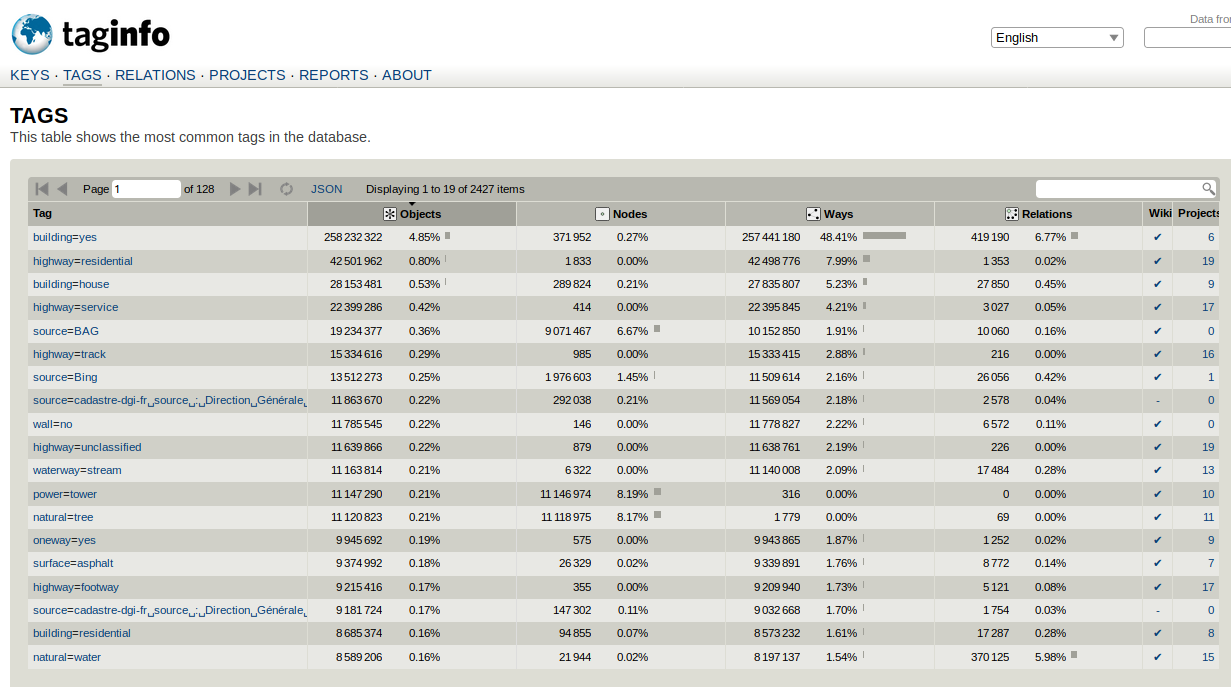
\includegraphics[width=0.9\linewidth]{Bilder/taginfo_example}
	\caption[Beispielhafte Darstellung taginfo]{Beispielhafte Datenbankeinträge der Datenbank von taginfo}
	\label{fig:taginfoexample}
\end{figure}
Leider stellten wir fest, dass die Beschreibungs-Einträge der Datenbank zu lückenhaft und damit für unsere Zwecke nicht geeignet sind.
Als Zwischenlösung kombinierten wir unseren bisherigen Ansätze, indem wir die Tag-Einträge der heruntergeladenen taginfo-Datenbank als Grundlage für ein Crawlen der OSM-Wiki-Seite verwenden wollten: Wir wollten ausnutzen, dass ein Link zu einer tag-beschreibenden Wiki-Seite die folgende Form aufweist:
\begin{center}
	\textbf{wiki.openstreetmap.org/wiki/Tag\%3\textit{Key}\%3D\textit{value}}
\end{center}
Wobei die Variablen \textit{key} und \textit{value} gemäß obiger Erklärung zu füllen sind. Unvorteilhafterweise stellte sich das Downloaden der Seiten schwieriger als gedacht heraus, da es zu manchen Tags noch nicht einmal eine Wiki-Seite gibt.

\subsubsection{Finallösung mit OSM-Wiki-Sitemap}
Schlussendlich verfolgten wir den finalen Ansatz, die aktuelle Sitemap der Wiki-Seite\cite{sitemap-index-wiki-link} herunterzuladen und anschließend die Links, welche die im vorhergehenden Abschnitt beschriebene Strukur ausweisten, herausgeschrieben.\\
Als Resultat hatten wir nun alle möglichen OSM-Wiki-Links lokal im \textit{txt}-Format zur Verfügung. Es konnten die Daten für den nächsten Arbeitsschritt, dem Aufbereiten der Einträge, weiterverwendet werden.
%TODO wir haben hier die Wiki-Seiten nicht herunterladen! nur die links in einer txt datei gehabt den export haben wir mit "export-links.py" gemacht

\subsection{Datenaufbereitung (Crawling)}
Eine Such-Engine auf Grundlage der HTMl-Files aufzusetzen, schlossen wir aus mehreren Gründen aus. Zuerst, findet sich in den HTMl-Files viele unnötige Informationen wieder, z.B. Bild-Links, \textit{JavaScript}-Teile oder gar unwichtige Metainformationen der Seite. Das alles verlangsamt zum einen die spätere Suche, verfälscht zum anderen aber auch den späteren Such- und Indizierungsprozess.\\
Unser Ziel war es, die Daten in eine solche Form umzuwandeln, dass unsere Such-Engine effizient darauf arbeiten kann.

\subsubsection{Initiale Idee}
Zu Beginn verfolgen wir die Idee, wiederkehrende Strukturen zu erkennen und in unser Suchranking miteinbeziehen. Existiert beispielsweise innerhalb der OSM-Wiki-Seite zu dem Tag \textit{highway=residential} ein Paragraphen \textit{related Tags} mit dem Eintrag \textit{highway=tertiary}, so ist es für den Nutzer möglicherweise interessant, auf Eingabe von \textit{highway} beide Ergebisse vorzufinden, auch wenn die Beschreibung von \textit{highway=tertiary} nicht allein zum Suchwort gepasst hätte. Es würde in folge dessen ein Beziehungs-Netzwerk aufgebaut werden.

\subsubsection{Probleme des initialen Ansatzes}
Unglücklicherweise stellten sich heraus, dass die Artikel des Wikis keiner spezifischen Form folgten. Zum einen sind die Strukturen zwischen den Artikeln sehr verschieden (zudem auch verschieden ausführlich), zum anderen finden sich inhaltlich ähnliche Absätze unter verschiedenen Überschriften, so beziehen sich ``See Also'', ``See also'', ``see also'', ``related tags'', ``Related Tags'' oder ``Similar Tag'' eigentlich semantisch auf dasselbe.
Das Ziel, weitere Informationen aus Tabellen zu entnehmen konnte aufgrund der heterogenen Struktur der Seiten ebenfalls nicht erreicht werden.

\subsubsection{Implementierte Variante}
%TODO wir haben die Wiki-Seiten herunterladen und in json abspeichern in einem Schritt gemacht. Weiter oben hattest du noch geschrieben, dass wir erstmal nur die html Seiten runtergeladen hatten.
Um die spätere Suchanfrage dennoch befriedigend beantworten zu können, einigten wir uns auf eine Struktur, die die Seite in drei Teile zerteilt. Später werden diese dann unabhängig voneinander durchsucht und gewichtet in die Ergebnisliste eingebracht. Die Struktur der aufbereiteten Daten lässt sich der unteren Grafik \autoref{fig:jsonDarstellung} entnehmen.\\
\begin{figure}[h]
	\centering
	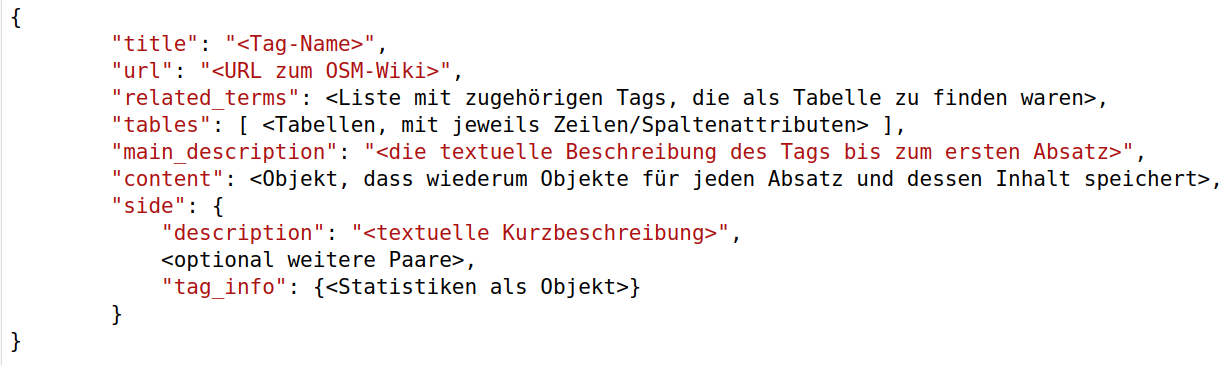
\includegraphics[width=0.9\linewidth]{Bilder/json_structure}
	\caption[Schematische Darstellung]{Schematische Darstellung der \textit{.json}-Struktur. Die Einträge mit spitzen Klammern markieren entsprech Meta-Anweisungen}
	\label{fig:jsonDarstellung}
\end{figure}
Das Ergebnis dieser Arbeitsphase war eine vollständige Liste von \textit{.json}-Objekten, die die texteullen Informationen der HTML-Seiten enthalten, Metainformationen wie Skripte und HTML-Tags jedoch nicht. Zudem sind die Informationen gruppiert und wir erhalten Zugriff auf die Auftrittshäufigkeit eines jeden Tags.

%TODO diese subsection
\subsection{ausführen}
%TODO zu crawling dazu machen, das
alle gesammelten link in die \texttt{links.txt} legen
\texttt{scrapy crawl osmWiki -t json -o keys.json}

\subsection{Suchanfrage beantworten}
Die finale Phase verknüpft alle bereits getätigten Arbeiten zu einer gesamten Anwendung, die aus mehreren funktionalen Einheiten besteht. Aus der \autoref{fig:implstructure} lassen sich die wesentlichen Komponenten erkennen. \\
Diese Dokumentation nutzt im Folgenden die Pipeline-artige Struktur der Implementierung aus, um die Implementierung von links her sequentiell zu erklären.

\begin{figure}[h]
	\centering
	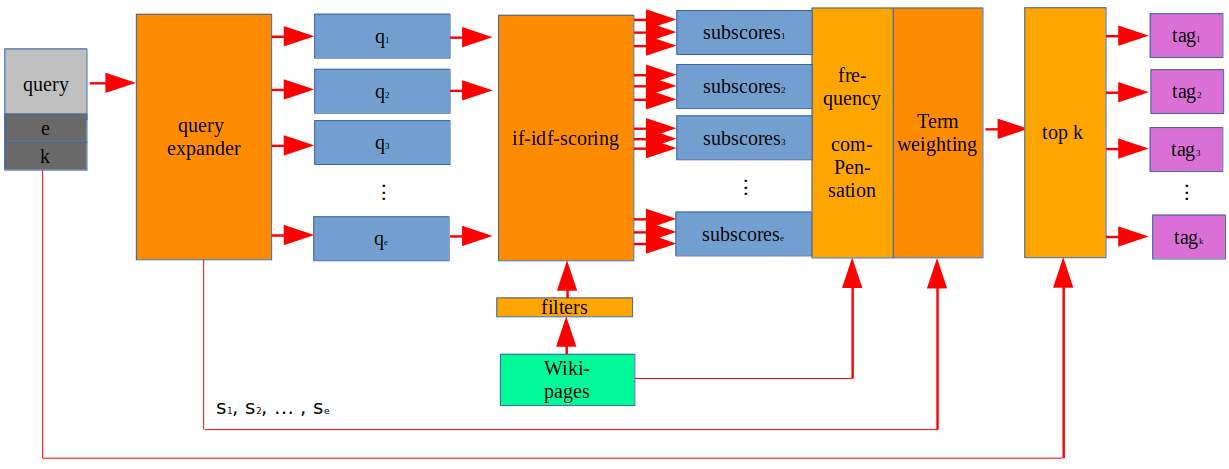
\includegraphics[width=1.0\linewidth]{Bilder/impl_structure}
	\caption[Schematische Darstellung]{Gesamtstruktur der Such-Implementierung}
	\label{fig:implstructure}
\end{figure}

\subsubsection{Eingabeparameter}
Die produzierende Ausgabe ist, neben den Wiki-Seite die den eigentlichen Suchraums überhaupt definiert, von drei Freiheitsgrade bestimmt. \\
Die \textit{query}-Eingabe besteht aus einem Wort der englischen Sprache, wie in  \autoref{sec:abgrenzung} zu Beginn definiert.
Die Ausgabe der Algorithmus soll $k \in \mathbb{N}_{>0}$ gültige Tags zurückliefern, die möglichst passend zur Eingabe \textit{query} sind. 
Wie wir in \autoref{sec:expansion} zeigen werden, erweitern wir die Eingabe als ersten Schritt semantisch. Der Grad Expansion wird durch den Parameter $e \in \mathbb{N}_{>0}$ beeinflusst.


\subsubsection{Query Expansion}\label{sec:expansion}
\textbf{Idee}\\
Die dahinterstehende Idee des ersten Pipeline-Knotens ist die Folgende: Da die Tag-Auswahl relativ begrenzt und zudem auf syntaktisch identische Treffer begrenzt ist, wollen wir die Eingabe erweitern. Dies möchten wir mit einem konstruiertem Beispiel verdeutlichen: Angenommen der User sucht nach \textit{Schnellrestaurant}, auf keiner OSM-Seite gebe es kein Vorkommen dieses Wortes, so würde die Suche keine Ergebnisse liefern. Durch Query-Expansion würden wir die Eingabe um die Wörter \textit{Fastfood-Restaurant}, \textit{Schnellrestaurants} und \textit{Restaurant} erweitern. Als Resultat können wir so \textit{amenity=fast\_food} erwarten. Ähnliche Beispiele könnten sich auch für die Englische Sprache konstruieren lassen.\\
\textit{}\\
\textbf{Realisierung}\\
Wir verwendeten für die Umsetzung das Framework \textit{Google word2vec}\cite{googleword2vec}. Es erlaubt auf Eingabe eines Wortes die Suche nach möglichst nahegelegenen Wörtern mit derselben Semantik. Der große Vorteil dadurch ist zusätzlich, dass wir parallel nach Singular und Plural der Eingabe suchen können, da deren Semantik praktisch identisch ist.\\
%TODO ich dachte wir haben e viele genommen nicht e-1
Das Resultat der Anwendung des Frameworks sind \textit{e-1} semantisch ähnliche Wörter, die zu dem Vektor der Eingabequery in nächster Umgebung lagen. Wir nennen diese im folgenden $q_2, q_3, \dots, q_e$. Implizit wird $q_1$ als die Anfangsquery betrachtet.

Neben den semantisch ähnlichen Queries speichern wir ebenfalls die vektorwertige (semantischen) Distanz zum Eingabevektor ab. Diese Ähnlichkeitswerte nennen wir entsprechend  $s_1, s_2, \dots, s_e$ mit der Eigenschaft $0 < s_i \leq 1$. Je höher dieser Wert, desto näher ist der Begriff der Ursprungsquery semantisch. Es dürfte offensichtlich sein, dass $s_1$ demnach den Wert $1$ besitzt.

\subsubsection{Scoring}\label{sec:scoring}
Die \textit{tf-idf-Komponente} ist dafür zuständig, möglichst relevante Tags zu den $s_i$ zu finden. Dafür nutzen wir die aufbereiteten \textit{.json}-Files des OSM-Wikis -  wie in \autoref{fig:jsonDarstellung} erklärt - als Grundlage für unsere Suche.
Die Bewertung besteht aus zwei Phasen, die sequentiell ausgeführt werden. In der ersten Phase werden zu einem gegebenen Suchwort jeweils 3 Scores berechnet. Jeder der drei Scores beschreibt hierbei den \textit{tf-idf}-Wert innerhalb eines Tag-Dokuments, repräsentativ für einen Dokumentteil.
Anschließend werden die Zwischenscores gewichtet verrechnet.
Zu Beginn erstellen wir drei verschiedene Indizes, die von dieselben Dimension sind. Der erste indiziert alle \textit{main-description}-Teile der Wiki-Seiten, der zweite alle \textit{side-description}-Teile und der letzte die restlichen Inhalte der \textit{.json}-Einträge. 
Für jedes der $q_i$ starten wir eine Suche in jedem Indizes, wir erhalten folglich die Zwischenergebnisvektoren $\vec{sub}_{i,0}, \vec{sub}_{i,1}, \vec{sub}_{i,2}$, stellvertretend für die drei Teile.\\
Die Idee war nun, eine sinnvolle Gewichtung der Treffer zu finden. Einen guten Treffer in der kurzen Main-Description soll in etwa so viel wert sein wie eine sehr passender Treffer in der ausführlichen \textit{Content}-Sektion. Somit soll es möglich sein, von der absoluten Textlänge zu abstrahieren und gleichzeitig sehr kurze Seiten, die dadurch einen sehr hohen tf-idf-Score haben, zu dämpfen.\\
In der Praxis stellte sich eine gleichmäßige Gewichtung von je ein Drittel als zweckmäßig heraus. Die neuen, kombinierten tf-idf-Scores lassen sich demnach mit $c_1 = c_2 = c_3 = \dfrac{1}{3}$ wie folgt berechnen:\\
\begin{center}
	$\vec{score}_{i} = \sum_{j=0}^{2} c_j * \vec{sub}_{i,j}$
\end{center}.

\subsubsection{Frequency Compensation}
Grundidee des \textit{Frequency Compensation} Moduls ist eine Bevorzugung oft genutzter Tags, gegenüber sehr seltenen. Hierzu beziehen wir die Statistik der in \autoref{sec:tagInfo} beschriebenen \textit{tagInfo}-Daten. \\
Da ein beispielweise zehnfach so oft getaggtes Wort, im Allgemeinen offensichtlich nicht auch zehnfach so relevant ist, verwendeten wir an dieser Stelle anstatt der reinen Multiplikation die Logarithmusfunktion. Die neuen Werte lassen sich mit 
\begin{center}
	 $\vec{score}_{i}^{'} = \vec{score_i} * log(\vec{freq})$
\end{center}
berechnen. $\vec{freq}$ bezeichnet hierzu den Vektor, der die absoluten Häufigkeiten der zugehörigen Tags beinhaltet. Selbige Konstruktion schließt offensichtlich den Fall aus, den Logarithmus von 0 zu berechnen.

\subsubsection{Term weighting}\label{sec:term_weighting}
Bis hierher wurden nun also zu einer Eingabe $e-1$ weitere Wörter abgeleitet, und jeweils gewichtete und anschließend geglättete tf-idf-Vektoren entsprechend berechnet. Als letzten Vorbereitungsschritt sollen die $e$ Vektoren zusammengelegt werden, gewichtet nach der ursprünglichen Relevanz zum Suchwort.\\
Die Bedeutung der Berechnung sollte intuitiv sein: Jeder der $e$ Vektoren speichert je einen Wert pro Tag ab, der die entsprechenden Relevanz abbildet. Die $s_i$, die ein Maß der semantischen Ähnlichkeit der Ursprungseingabe $q_1$ zu allen anderen $q_i$ sind, Werden nun als Gewichtung verwendet. Dadurch werden semantisch ähnliche Suchtreffer höher gewichtet als semantisch suboptimale. Ein Beispiel sollte dies klar machen. Angenommen, die Suche nach $q_1 =$ \textit{waterfall} wird zu $q_2 =$ \textit{rural\_area} mit einer Ähnlichkeit von  $s_2 = 0.3$ expandiert und dessen if-idf-Score des Wertes \textit{residential=rural} wäre 200. Zudem habe $q_1 $ einen unerwartet niedrigen if-idf-Score von 120 beim Tag \textit{waterway=waterfall}, da z.B. die Wiki-Seite unbefriedigend erstellt worden ist. Durch die Gewichtung der Vektoren gemäß semantischer Ähnlichkeit zur ursprünglichen Eingabe, erhalten wir den erwarteten Suchtreffer.\\
Der finale Scoring-Vektor lässt sich demnach mit\\
\begin{center}
	$\vec{fin} = \sum_{i=1}^{e} s_i * \vec{score}_{i}^{'}$
\end{center}.
berechnen.


\subsubsection{top k - result collecting}
Die Berechnung in \autoref{sec:term_weighting} liefert uns eine Vektor mit der Dimension in der Anzahl der Tags, und repräsentiert die Befriedigung der Eingabequery. Um den Benutzer eine Auswahl über mehrere mögliche passende Tags zu bieten, werden nun davon die besten \textit{k} Ergebnisse zurück geliefert.
%TODO wir suchen argmax und geben den, Tag aus unserem index aus.

\section{Bedienung der Anwendung}

\subsection{Starten}
man muss im gleichen ordner auch \texttt{GoogleNews-vectors-negative300.bin}, das hier runtergealden werdxen kann \cite{googleword2vec} und die \texttt{tags.json} von uns aus dem crawler.\\
\texttt{python3 ./search.py}
%TODO ausformulieren
\subsection{Aufbau der Anfrage}
Beispiel Anfrage
\begin{lstlisting}
	curl -d '{"query":"house", "amount":5, "nearest_neighbor":10}' -H "Content-Type: application/json" -X POST http://localhost:8080
\end{lstlisting}
%TODO ausformulieren
\subsection{Rückgabe}
\begin{lstlisting}
	[["Tag:landuse=residential", 0.6396545082270853], ["Tag:building=house", 0.11751306010961371], ["Tag:building=cabin", 0.09408986107578671], ["Tag:building=detached", 0.07558317020115245], ["Tag:building=farm", 0.07315940038636194]]
\end{lstlisting}
%TODO ausformulieren

\section{Projektrefelxion}
\subsection{Verbesserungsansätze}
Nach Abschluss des Projektes möchten wir ein paar Ansätze nennen, an denen man in Zukunft arbeiten könnte, um das System effizienter und schneller zu machen und die Qualität des Rankings zu erhöhen.
\subsubsection{Google Word2Vec}
Das aktuelle Modell, das wir für das Expandieren der Wörter auf e Terms verwenden, besitzt eine Größe von circa 3.4 Gigabyte. Folglich nimmt das Starten des Serves eine erhebliche Zeit in Anspruch, zudem werden Speicherressourcen verschwendet.\\
Da in dem eigentlichen tf-idf-Scoring ein Treffer nur als ein solcher gezählt wird, wenn dieser als String innerhalb eines Wiki-Dokumente auftaucht, könnten wir in dem Google-Vektor Modell nur solche Wörter als Eingabe erlauben, die in der Wiki-Seiten vorkommen.\\
Das spart Platz im RAM, sowie Zeit beim Ein- und auslesen.
%TODO auslesen macht kein sinn. aber vor allem wird das Suchen extrem viel schneller.
\subsubsection{Syntaktische um Semantische Suche ergänzen}\label{sec:semantikInSuche}
Wir verwenden eine semantische Erweiterung der Startanfrage auf insgesamt \textit{e} Suchanfragen. Leider verwendet unser aktuelles System für den eigentlichen Suchalgorithmus lediglich eine syntaktische Suche. Hier entstehen Treffer, die nicht als solche gezählt werden sollten. Beispielsweise wird ein Tag bei der Suche nach \textit{waterfall} mit einem Treffer markiert, wenn es Formulierungen wie \textit{`... not to be confounded with waterfall''} beinhaltet.\\
Man könnte sich in diesem Zusammenhang mit dem Framework \textit{NLTK} unter Python auseinandersetzen. Hier könnte neben der Wiki-Seiten, auch die Query semantisch analysiert werden, sodass gezielt Fragen beantwortet werden könnten
\subsubsection{Struktur besser ausnutzen}
In Anlehnung an \autopageref{sec:semantikInSuche}, wird in unserem Modell die interne Struktur der Wiki-Seiten noch nicht ausreichend genutzt. Man könnte noch mehr Semantik aus der Struktur den Seiten entnehmen, indem beispielsweise Tabellen besser eingebunden werden. \\
Schwierig bleibt jedoch auch hier wieder die Gewichtung der Semantik. Selbiges Problem wird in \autoref{sec:gliederungContent} diskutiert.
\subsubsection{Gewichtung der Content-Teile}
\label{sec:gliederungContent}
In \autoref{sec:scoring} erläuterten wir das Vorgehen, verschiedene Teile der Wiki-Seiten unabhängig zu indizieren und anschließend den Score geeignet zu kombinieren. Eine begründete Wahl der $c_i$ zu finden, stellt sich als Herausforderung dar. Der Lesen möge sich die Frage ``Welcher Tag passt am besten zur Eingabe ...?'' konstruieren, um herauszufinden, welche Parameterwahl als passend erscheint. \\
Für mehr als 2 Freiheitsgrade der Parameter wird es sich allerdings als schwierig herausstellen, die Optimalität dieser Wahl zu begründen.

%TODO softmax ausgabe noch beschreiben warum


\subsection{Ergebnisqualität}
Dieser Abschnitt erläutert anhand ausgewählter Anfragen die Charakteristika der entwickelten Such-Engine. Dieser Abschnitt kann unter anderem auch Inspiration für weitere Verbesserungen verstanden werden.
\subsubsection{gute Ergebnisse}
\begin{minipage}[t]{0.45\linewidth}
\begin{lstlisting}
	Search: airport
	Tag:aeroway=terminal
	Tag:aeroway=apron
	Tag:aeroway=gate
	Tag:aeroway=taxiway
	Tag:aeroway=hangar
\end{lstlisting}
\end{minipage}
\begin{minipage}[t]{0.45\linewidth}
\begin{lstlisting}
	Search: cloths
	Tag:shop=dry_cleaning
	Tag:shop=laundry
	Tag:shop=clothes
	Tag:amenity=lavoir
	Tag:shop=fabric
\end{lstlisting}
\end{minipage}
\\
\begin{minipage}[t]{0.45\linewidth}
	\begin{lstlisting}
	Search: ball
	Tag:sport=table_tennis
	Tag:sport=boules
	Tag:sport=tennis
	Tag:sport=beachvolleyball
	Tag:sport=lacrosse
	\end{lstlisting}
\end{minipage}
%TODO so gut?

\subsubsection{überraschende Ergebnisse}
\begin{minipage}[t]{0.45\linewidth}
\begin{lstlisting}
	Search: subway
	Tag:railway=subway_entrance
	Tag:station=subway
	Tag:railway=subway
	Tag:public_transport=platform
	Tag:amenity=fast_food
\end{lstlisting}
\end{minipage}
\begin{minipage}[t]{0.45\linewidth}
\begin{lstlisting}
	Search: knight
	Tag:castle_type=defensive
\end{lstlisting}
\end{minipage}
%TODO beschreiben warum
\subsubsection{unzureichende Ergebnisse}
\begin{lstlisting}
	Search: bow
	Tag:sport=bandy 	 	0.5166928762734
\end{lstlisting}
aber
\begin{lstlisting}
	Search: arrow
	Tag:sport=archery 	 	0.35975876802262186
	Tag:natural=ridge 	 	0.1781519400540717
	Tag:guidepost=simple 	 	0.17534783227284406
	Tag:highway=traffic_signals 	0.14598696420532248
	Tag:junction=roundabout 	0.1407544954451397
\end{lstlisting}
%TODO es gibt also archery, wird bei bow aber nicht gefunden
\begin{lstlisting}
	Search: church
	Tag:tower:type=bell_tower 	 	0.5335585869452344
	Tag:denomination=mormon 	 	0.2835628039185601
	Tag:landuse=churchyard 	 		0.15180475416031017
	Tag:building=cathedral 	 		0.02060323943121495
	Tag:amenity=place_of_worship		0.010470615544680439
\end{lstlisting}
aber
\begin{lstlisting}
	Search: building chruch
	Tag:building=church 	 		0.3497134817186539
	Tag:building=barn 	 		0.19188670466761262
	Tag:building=mosque 	 		0.1561445060806261
	Tag:building=farm_auxiliary 		0.1543794781358878
	Tag:building=construction 	 	0.14787582939721966
\end{lstlisting}
%TODO findet es nicht direkt, auch wenn es das gibt

\section{ausblick/besser machen}
- automatische Korrektur, wenn man sich verschreibt. "airprt" wird zu "airport"
%TODO ausformulieren


\section{notizen}
Phase 1: Planung
- Tags und dazugehörige semantische Beschreibung holen
- in Struktur bringen
- Suchanfrage an Daten 
- gensim (Python von Mendel zu Beginn vorgeschlagen)
- vorhanden/nicht vorhanden 
-> bewerbung fehlt
- tf-idf
-> gut, aber Problem: Mehrere Links auf dieselbe Seite
-> Duplikate entfernen
-> hohe Gewichtung für kleine Seiten
-> Multiplizieren mit log/oder Wurzel 2
- Suchraum expandieren
- mit Google Modell Anfrage semantisch auffüllen, Suche durchführen, am meisten Relevanten herausnehmen.


\pagebreak
\section{Vorgehensweise}

1. Anschauen von wiki xml dump (Export von 2013) 
-> Struktur nicht erkennbar + veraltete Daten.

2. taginfo: (um an Tags zu kommen) Datenbank herunter geladen, nicht immer aktuellster Stand, Statitsik: Idee: Generieren von Links, mithilfe von Key=value Anfrage an Website, aber möglicherweise Fehler, da dazu kein Wiki-Eintrag exisitert.

3. nochmal wiki xml dump -> Alle Links des Wikis
4  davon Struktur: filtern der Links, die auf Tags verweisen.
-> Ergebnis: Liste aller Links, die auf OSM-Tag-Seiten zeigen.
5. Crawler: Download aller HTML Files
6. Ergebnis: pretty-Datei.

Implementierung:
1. Schritt: expandieren der Suchanfrage gemäß Semantik auf k Begriffe (mithilfe von W2V) 
2. Schritt: für jeden 


herunterladen der tags: https://taginfo.openstreetmap.org/


\section{Dependecies}
%TODO mitliefern?
\begin{itemize}
	\item crawler: Scrapy(crawl) und BeautifulSoup(html-parser)
	\item suche: sklearn(tfidf), gensim(google-model), numpy und nltk(für stopwords)
\end{itemize}

\pagebreak
\section{Anhang}


\bibliographystyle{unsrt}
\bibliography{lit}

\end{document}